\chapter{Other energy terms also considered}

In this section, our attempts to fold struc

\section{Evolutionary distance constraints}

\begin{figure}
    \centering
    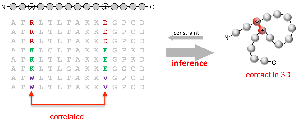
\includegraphics[width=0.85\textwidth]{figures/evo_constraint.pdf}
    \caption{Evolutionary constraints}
    \label{fig:evo_constraint}
\end{figure}

As discussed previously, it is increasingly difficult to obtain sufficient distance restraints as the size of the protein increases.
A recently developed methodology uses sequence analysis to infer residue contacts in 3D space. 

In brief, the method works by identifying sequence co-variation, which retains favorable contacts between residues.
This way, pair of residues which are probable to be close in 3D space can be identified.
The procedure is briefly summarized in Fig.~\ref{fig:evo_constraint}.

In this proof-of-concept study, 270 contacts were obtained a multiple-sequence alignment using the EVfold program (Wouter Boomsma, personal communications) for the 269 residue protein Savinase.
The restraints were simply treated as NOE restraints using existing code.
A similar simulation to that which folded Rhodopsin was adopted. 
In terms of computational resources, these were increased to 100 threads and $75 \times 10^6$ iterations, compared to only 72 threads and $50 \times 10^6$ iterations for the Rhodopsin simulation.
One thread identified a native-like structure.

The folding simulation yielded a lowest energy 


% \begin{figure}
%     \centering
%     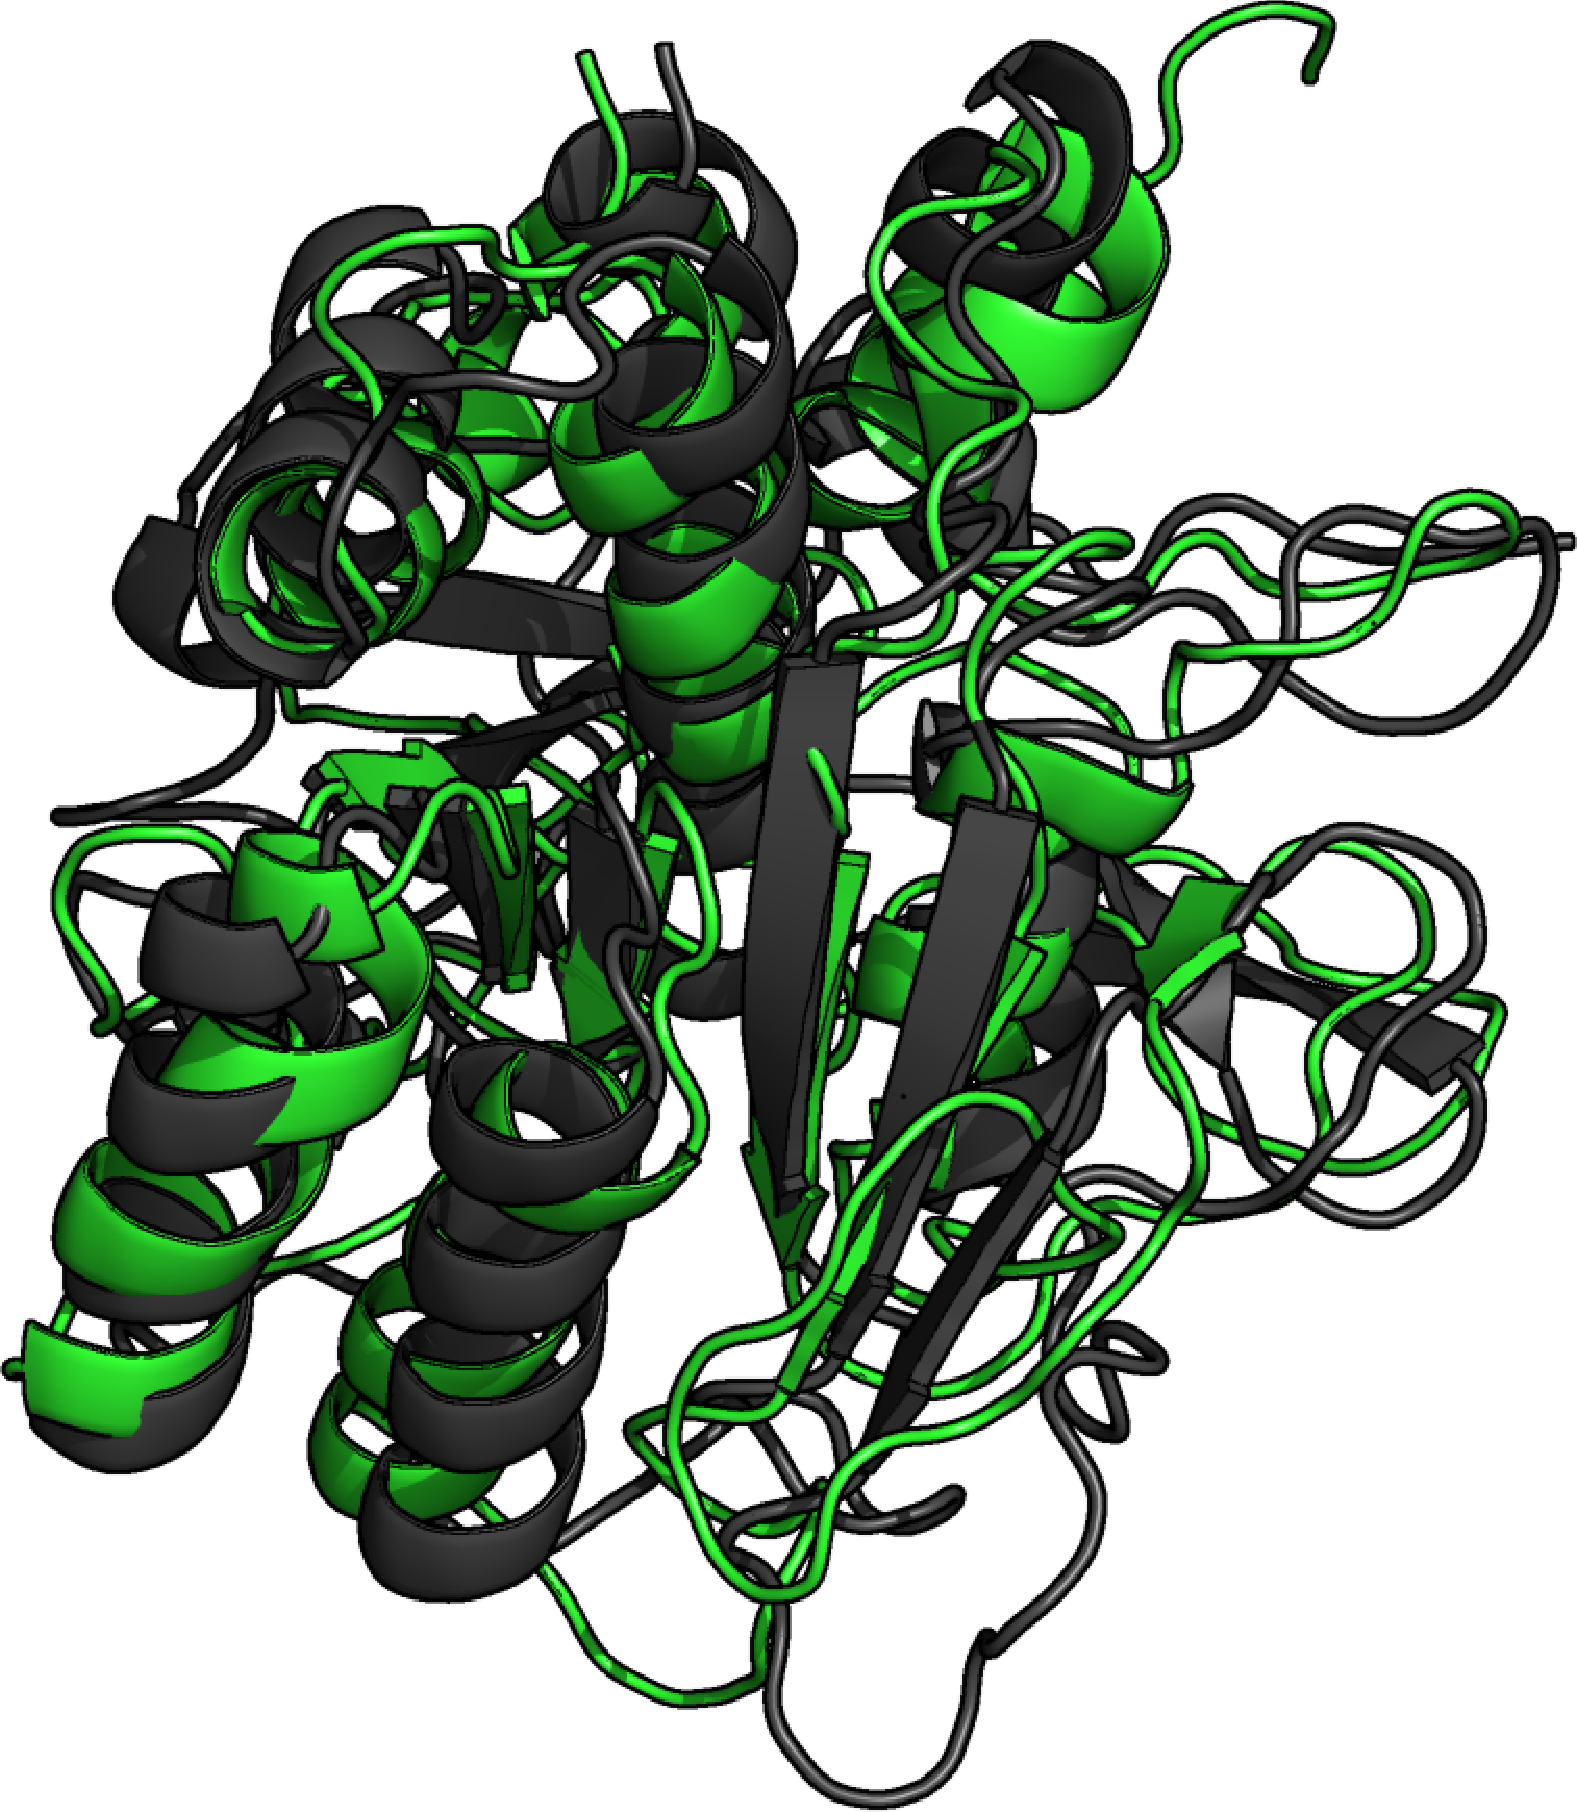
\includegraphics[width=0.60\textwidth]{figures/savinase_fold/savinase_lowest_e.pdf}
%     \caption{The lowest energy structure of Savinase after the refinement (green) and the 
%              1SVN crystal structure (grey). The CA-RMSD is 2.9 \AA.}
%     \label{fig:savinase_align}
% \end{figure}



\begin{figure}%
    \centering
    \subfloat[Lowest RMSD sample]{
        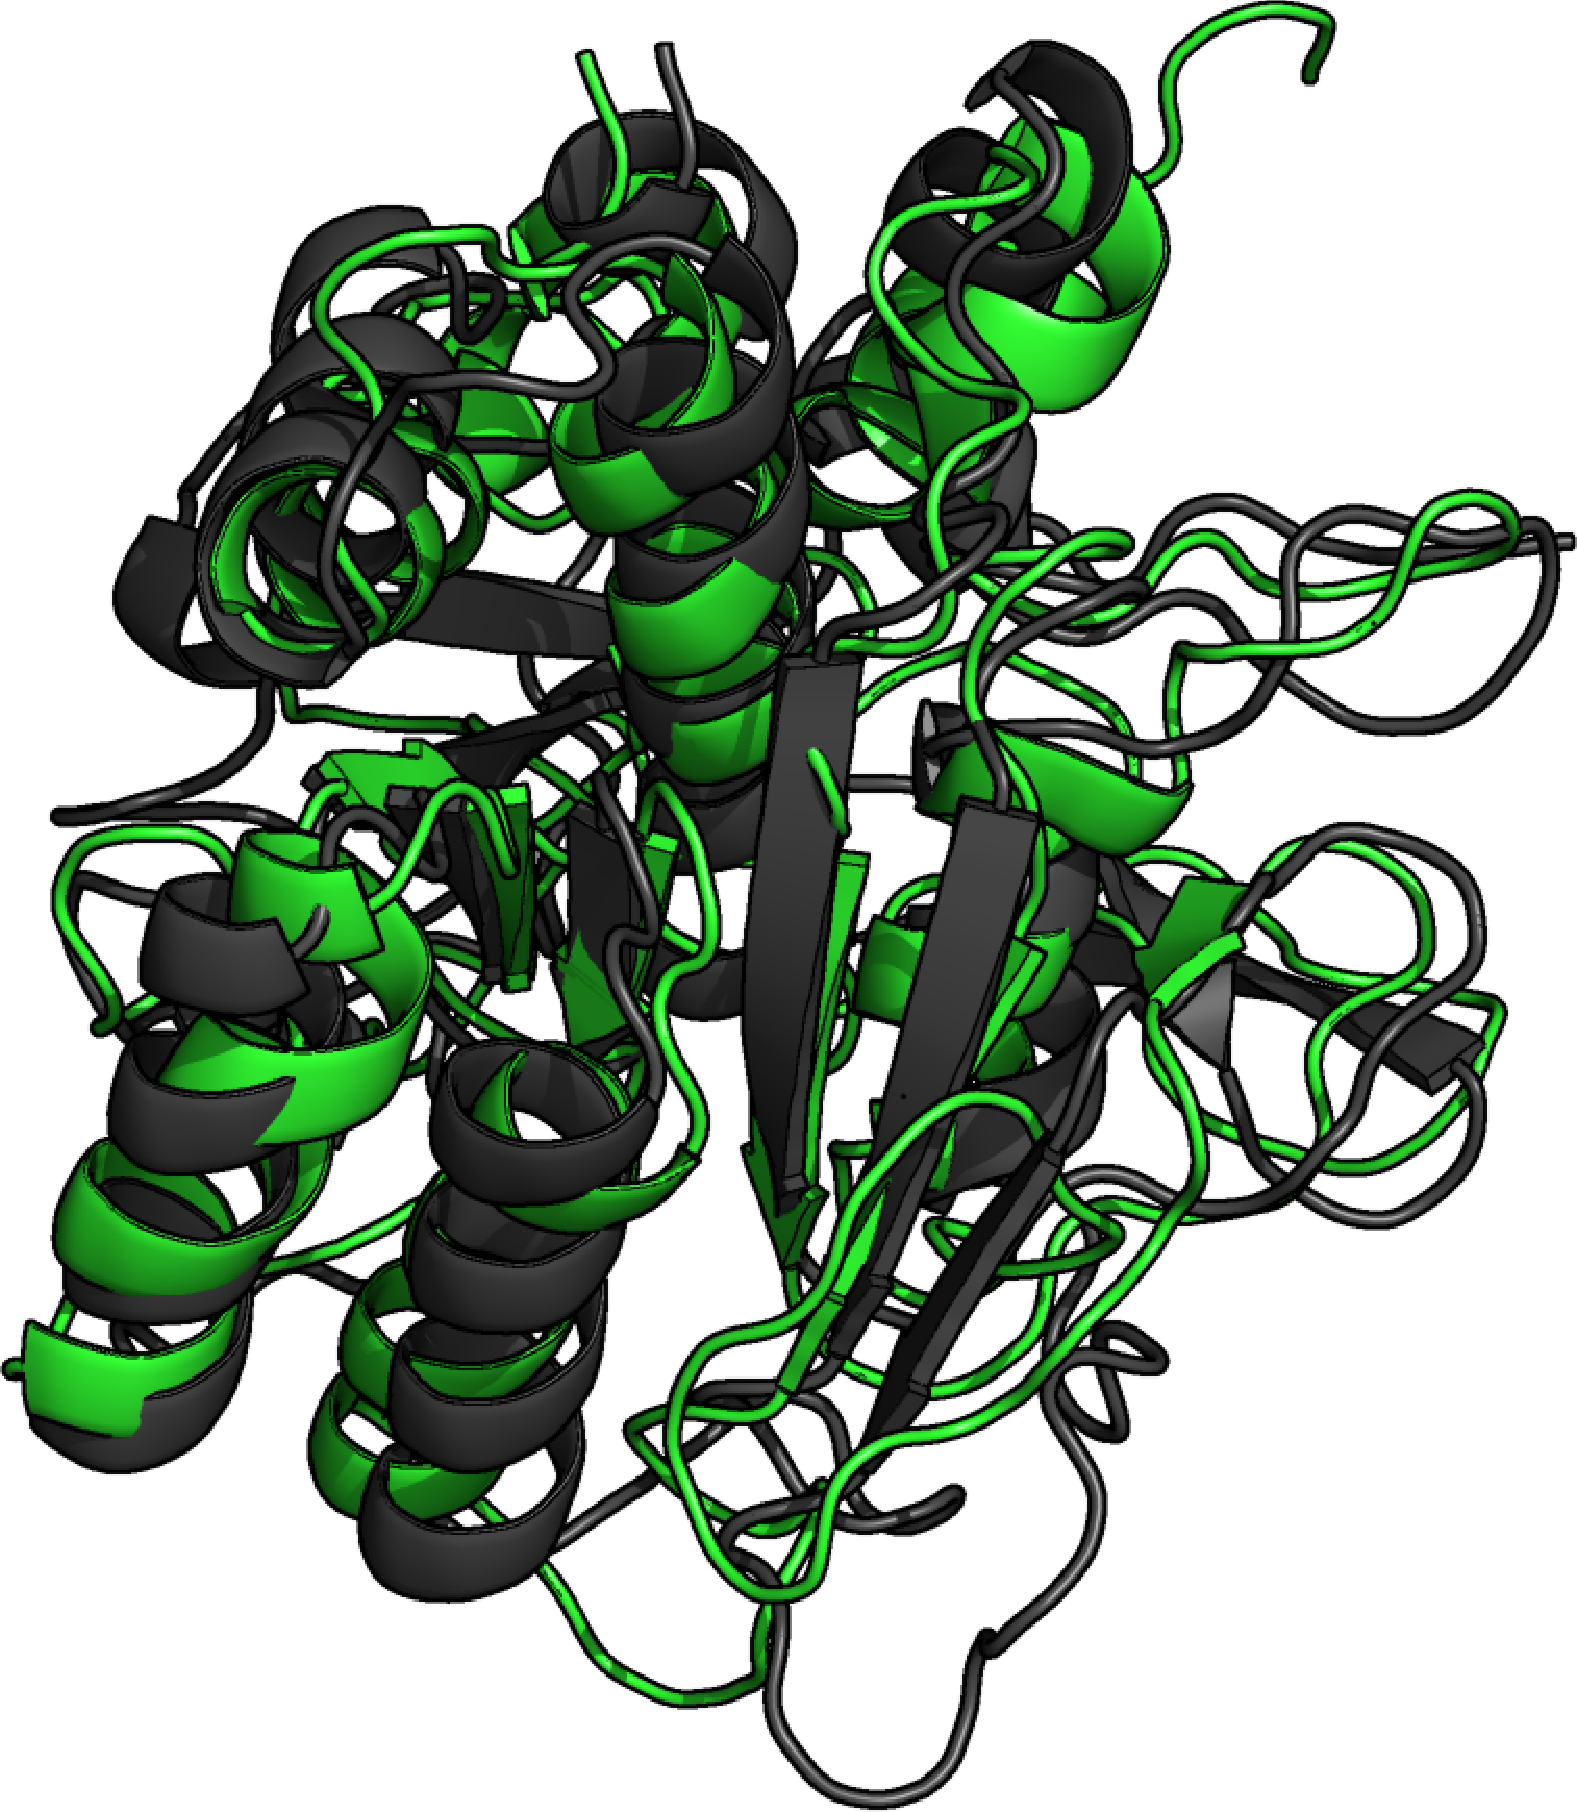
\includegraphics[width=0.40\textwidth]{figures/savinase_fold/savinase_lowest_e.pdf}
        %{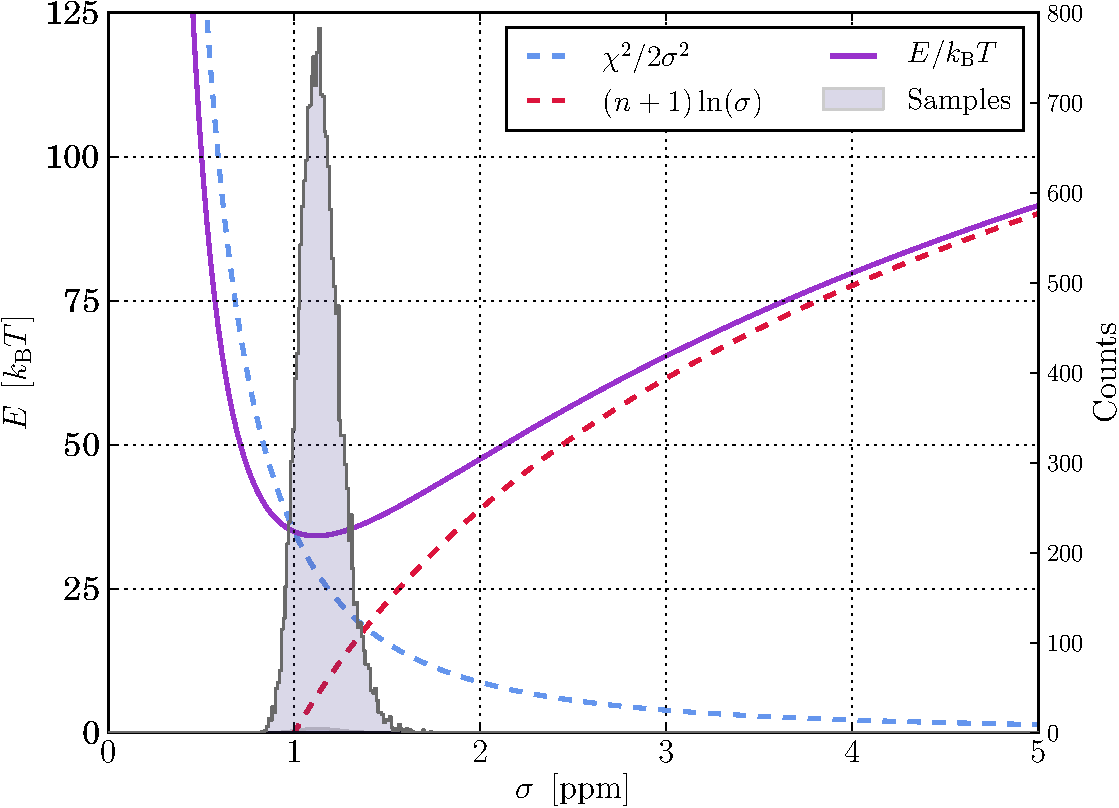
\includegraphics[width=0.42\textwidth]{sigma_prior.pdf} }
    }
    \subfloat[Lowest energy sample]{
        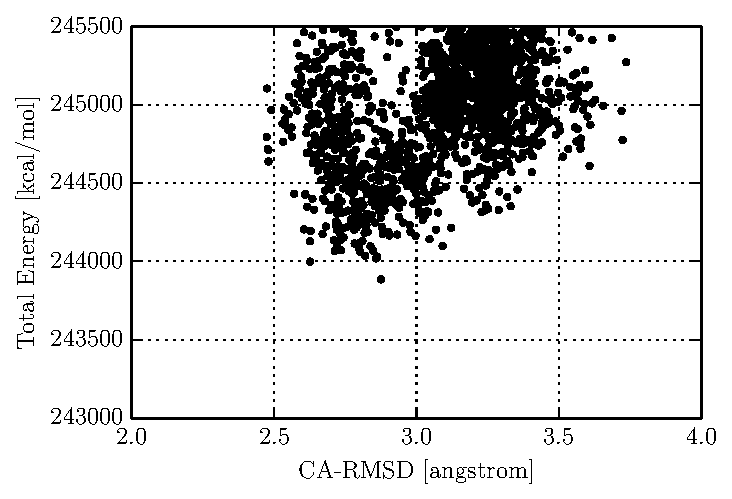
\includegraphics[width=0.60\textwidth]{figures/savinase_fold/savinase_refinement.pdf}
    }
    \caption{Sampling of $\sigma$ and $\gamma$ for 2OED for Ca-chemical shifts. $n = 55$ and $\chi^2 = 69.7$.}
    \label{fig:savinase_fold}%
\end{figure}


% 
% \begin{figure}
%     \centering
%     \caption{Savinase folded}
%     \label{fig:savinase_align}
% \end{figure}
% 



%Distance constraints from evolutionary sequence comparison
%To supplement NMR data for larger proteins we exploit recent breakthroughs in our ability to understand quantitatively the constraints on structure observed through evolution. More precisely, it is now possible to predict with sufficient accuracy whether amino acids are spatially close to one another in a protein structure by looking at the co-variation of amino acids during evolution (Marks et al. 2011). In a proof-of-concept study we used this approach to predict 270 contacts from a multiple sequence alignment of the 269-residue long enzyme Savinase. When used in a simulation protocol together with backbone chemical shifts we obtained a X Å structure (Figure 3c), corresponding to one of the most accurate NMR structures of a large protein obtained using only chemical shifts.

\chapter{Mass-spectroscopy in protein structure determination}

This section introduces the two experimental methods, hydrogen exchange mass spectroscopy (HXMS) and cross-correlation mass spectroscopy (XCMS), and possible application in protein folding.

These experimental methods are attractive, since the experiments are relatively easy to carry out.

mass spectroscopy 

\section{Cross-linking mass spectroscopy (XLMS)}


XLMS has previously been used to 

We considered several linkers of different lengths. The \textit{de facto} standard linkers, DSS and DST which measure 11 \aa ngstr\"o m and 6.4 \aa ngstr\"o m, respectively.

\begin{figure}
    \centering
    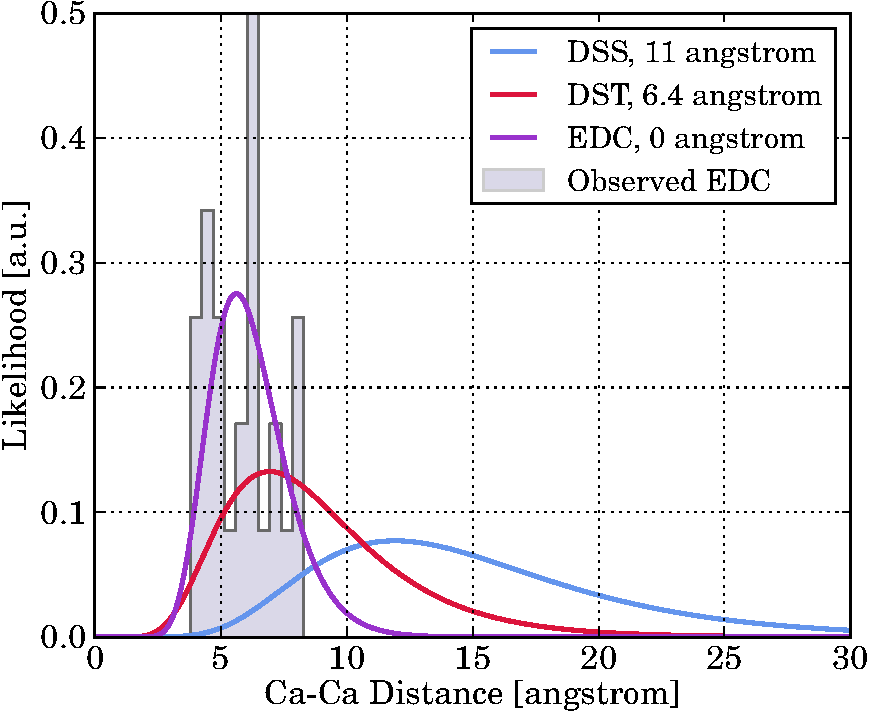
\includegraphics[width=0.65\textwidth]{figures/xcms/lognormal.pdf}
    \caption{linkers}
    \label{fig:linkers}
\end{figure}


\begin{figure}
    \centering
    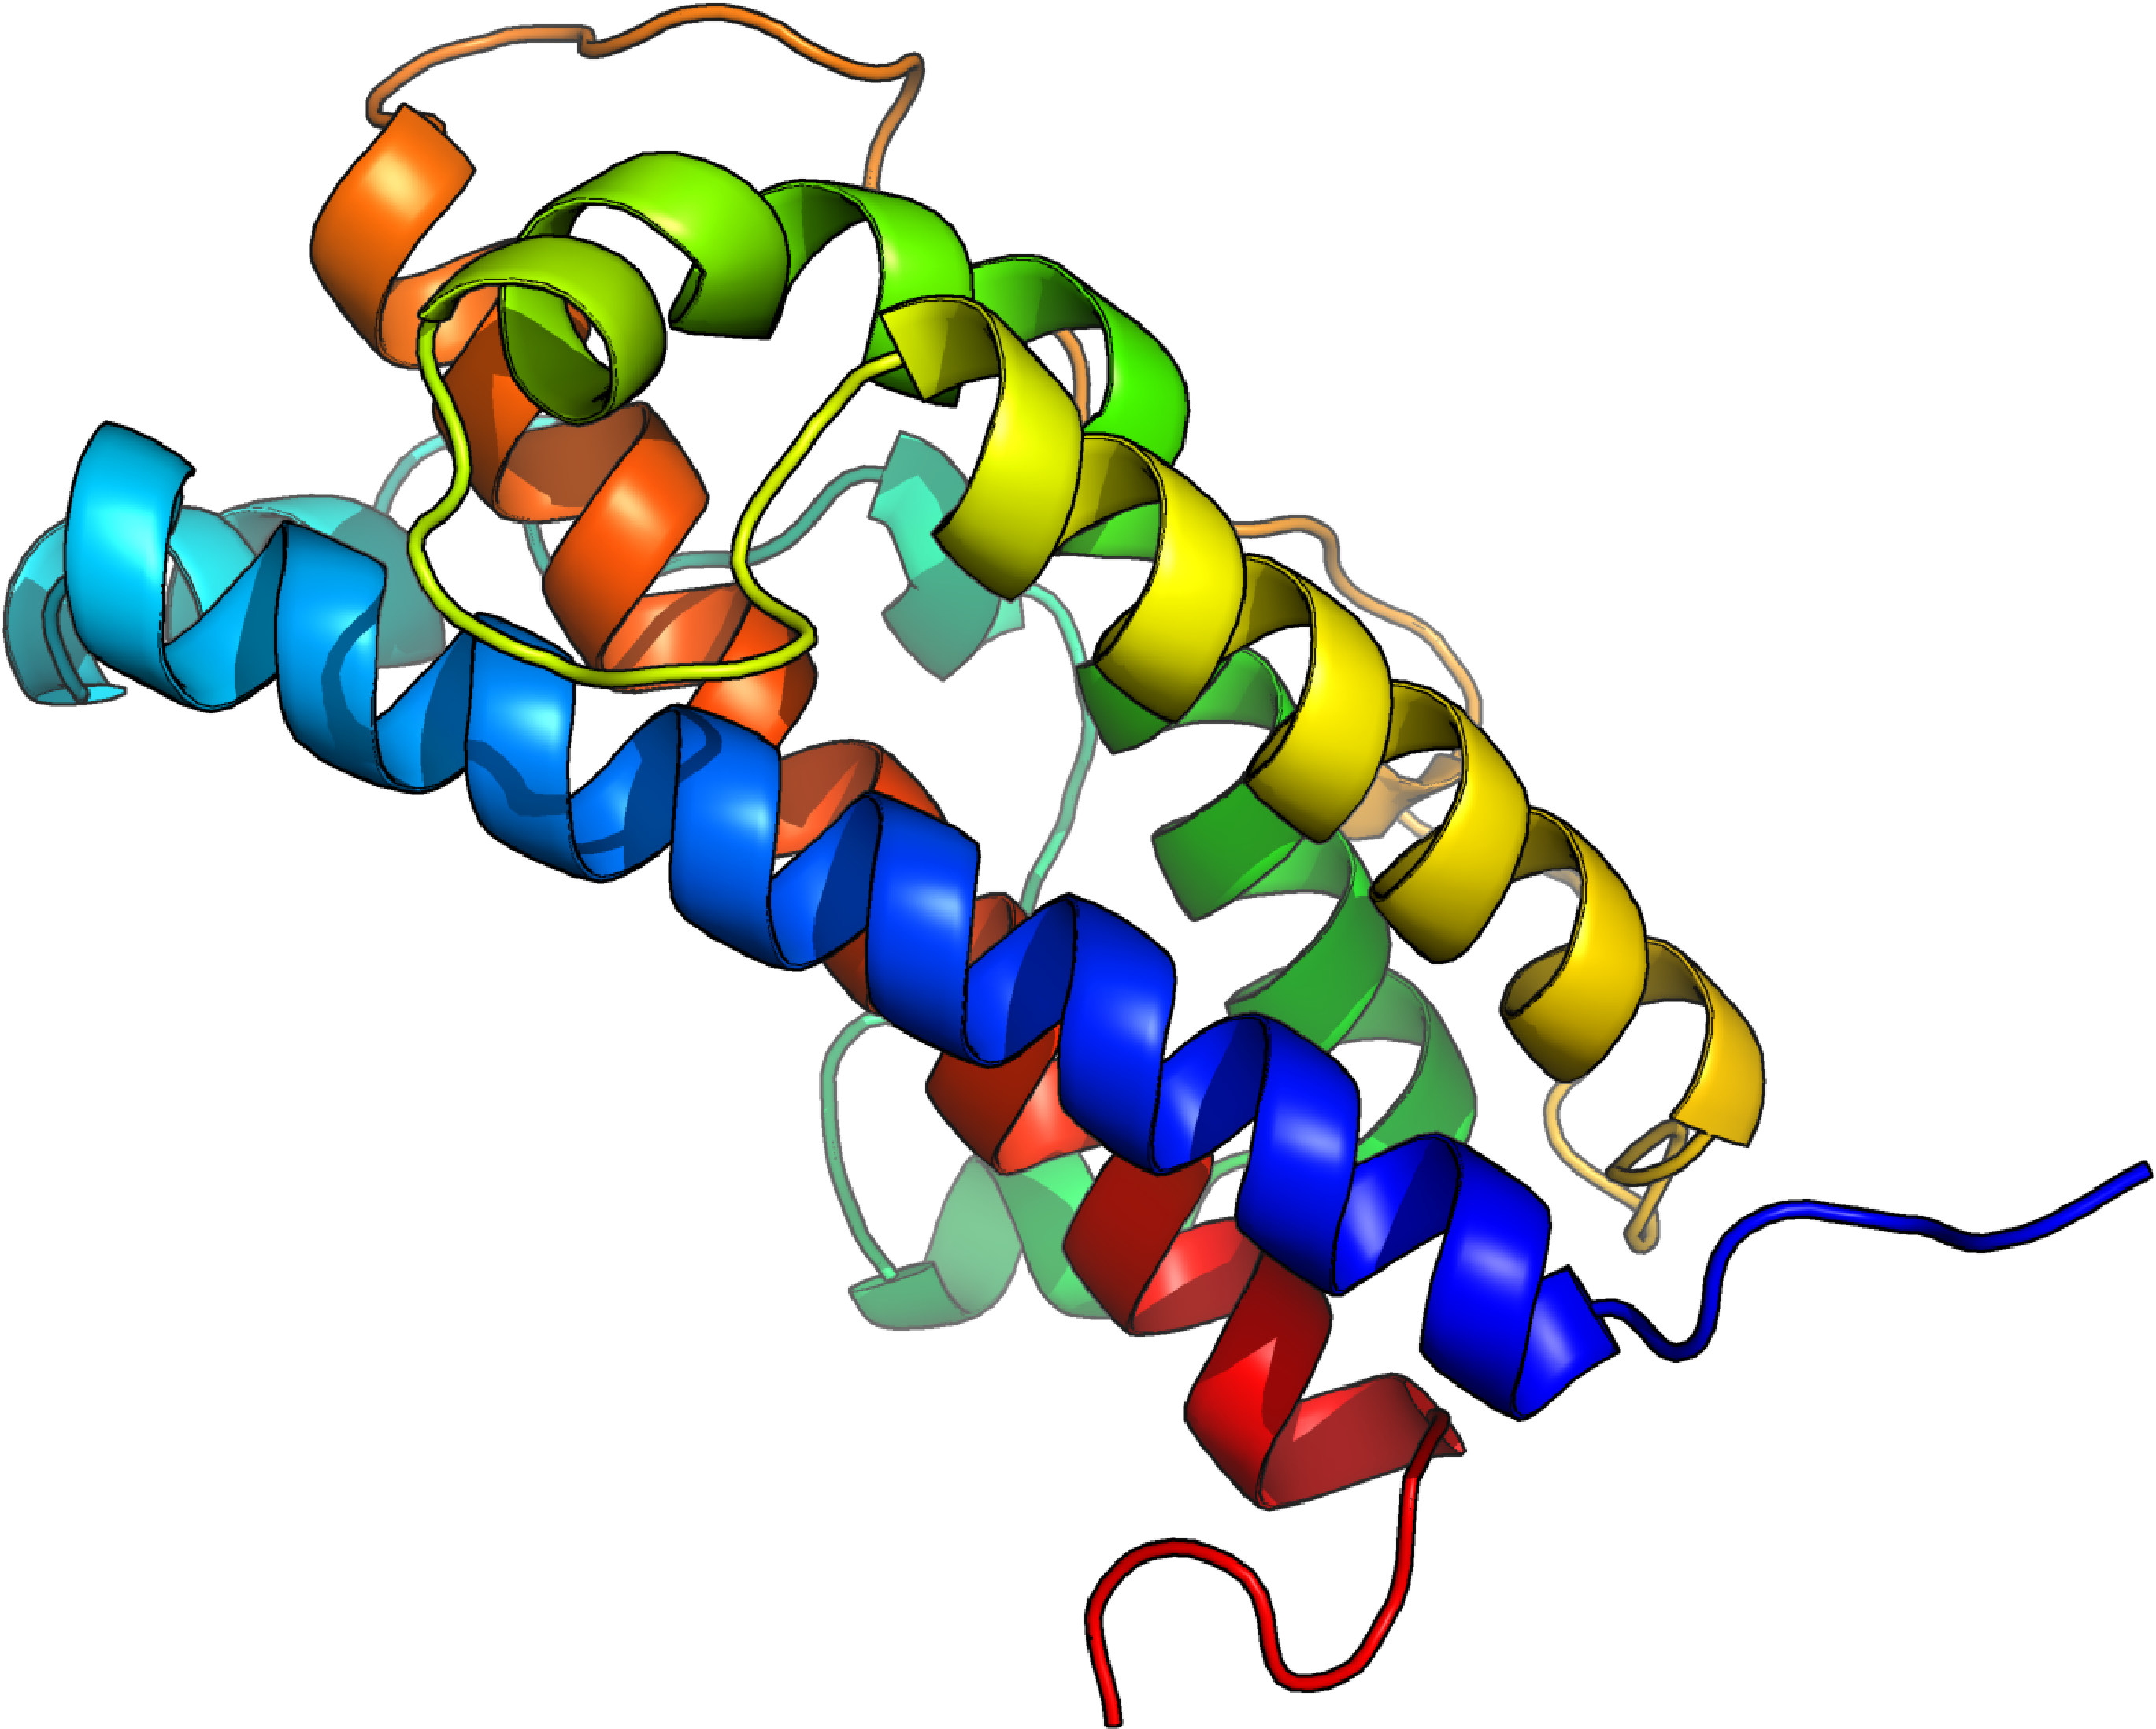
\includegraphics[width=0.85\textwidth]{figures/hGH_rainbow.pdf}
    \caption{linkers}
    \label{fig:hGH_homology}
\end{figure}

\section{Hydrogen exchange mass spectroscopy (HXMS)}

\subsection{Hydrogen bond criterion}

The interresidue hydrogen bond criterion of the DSSP program\cite{dssp} is used to identify hydrogen bonds.
The DSSP program uses an electrostatic model, assuming partial charges of -0.42 e and +0.20 e to the carbonyl oxygen and amide hydrogen respectively, and -0.42 e and +0.20 e to the carbonyl carbon and amide nitrogen, respectively.
A hydrogen bond is empirically defined as having an interaction energy given as
\begin{equation}
E_\mathrm{HB} = \left(\frac{1}{r_\mathrm{ON}} + \frac{1}{r_\mathrm{OH}} - \frac{1}{r_\mathrm{CH}} - \frac{1}{r_\mathrm{CN}} \right)\cdot\ 27.89\ \mathrm{kcal/mol}
\end{equation}
stronger than a cut-off of -0.5 kcal/mol.

\subsection{Beta-binomial model}
The likelihood model that correlates a measured deuterium uptake to an integer number of hydrogen bonds in a strand is a simple model based on a beta-binomial distribution.

\begin{equation}
P(N_\mathrm{HB} = k | \alpha, \beta) = \binom{n}{k} \frac{B(k+\alpha, n - k + \beta)}{B(\alpha, \beta)}
\end{equation}
where $n$ is the length of the strand (i.e. the maximum possible number of hydrogen bonds), $N_\mathrm{HB}$ is the number of observed hydrogen bonds and $k \in {0, ... ,n}$ are the possible values of $N_\mathrm{HB}$. $\alpha$ and $\beta$ are variables and $B(x,y)$ is the beta-function given as:
\begin{equation}
B(x,y)=\frac{(x-1)!(y-1)!}{(x+y-1)!}
\end{equation}
The mean, $\mu$, and variance, $\sigma^2$, and variance of the beta-binomial distribution is
\begin{eqnarray}
    \mu      & = & \frac{n\alpha}{\alpha + \beta}\\
    \sigma^2 & = & \frac{n\alpha\beta(n + \alpha + \beta)}{(\alpha + \beta)^2(1 + \alpha + \beta)}
\end{eqnarray}
If $\mu$ and $\sigma^2$ are estimated, then $\alpha$ and $\beta$ can then be derived for a strand of length $n$ as:
\begin{eqnarray}
    \alpha & = & -\frac{\mu(\mu^2 - \mu n + \sigma^2)}{\sigma^2 n + \mu^2 - \mu n}\\
    \beta  & = & \frac{n\alpha}{\mu} - \alpha
\end{eqnarray}


\subsection{HXMS likelihood function}

The simplified forward-model that correlates the protein structure, $\mathbf{X}$ to the measured values of deuterium uptake, $\{D_i\}$ is obtained by constructing an empirical function $f(D_i) \mapsto \mu$











